\chapter{\label{chapter:Moderator}The Moderator}

The entry point into GMAT's engine is the Moderator.  The Moderator controls program flow, creating
components through the factory manager that are then managed in the configuration manager, and
then using these components to model missions in a sandbox.  The Moderator creates the engine
components, manages those components when necessary, and controls the processes in GMAT's engine. 
It initializes the Sandbox prior to a run, and launches the run in the Sandbox.  In other words, the
Moderator is the central control element of GMAT, acting as the interface between users and the
internal elements of the system, and facilitating communications between those internal elements.

The engine contains one component, the Publisher, that does not interact with the Moderator beyond
initialization.  The Publisher, described in Chapter~\ref{chapter:Publisher}, is the communications
interface between the Sandbox objects and the Subscriber objects that present data to users.  The
following sections discuss interactions between engine components and the Moderator.With the
exception of initialization, these interactions exclude the Publisher.

This chapter explains how the Moderator accomplishes its tasks.

\section{Moderator Design Principles}

Figure~\ref{figure:GMATStackDiagram} shows a high level view into GMAT's architecture.  That figure
contains arrows showing all of the allowed communications paths in the engine.
Figure~\ref{figure:ModeratorInteractions} shows the portion of that diagram that corresponds to the
Moderator's role in GMAT.  The Moderator handles all communications between the Interpreters and
the engine, and between the components of the engine used to set up and run a mission.

\begin{figure}[htb]
\begin{center}
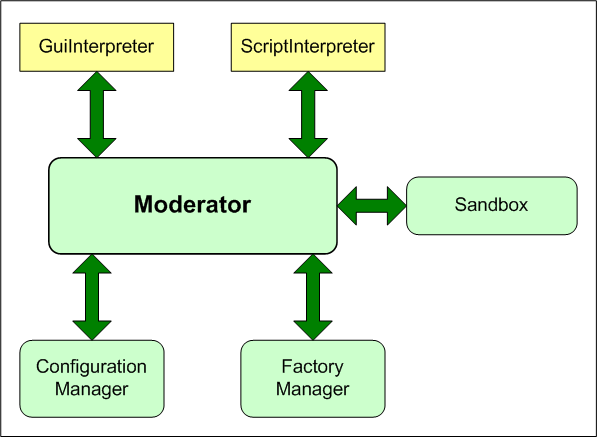
\includegraphics[239,175]{Images/ModeratorInteractions.png}
\caption{Program Flow and the Moderator}
\label{figure:ModeratorInteractions}
\end{center}
\end{figure}

While the arrows in this figure show the information flow through the Moderator, they do not state
explicitly what data or objects move along these paths.  The Moderator is the manager for all of
the tasks accomplished in the engine.

The Moderator design is built around two design patterns: the Singleton pattern and the Mediator
pattern.  The Mediator pattern is discussed in Section~\ref{section:ModeratorMediator}.  The
Moderator consolidates the management actions needed for GMAT into a central location.  It is a
singleton to ensure that this consolidation happens at only one place for the GMAT executable.  Each
instance of GMAT running in memory has exactly one Moderator managing the GMAT engine.

There are seven key actions that the Moderator is responsible for managing, described in the next
section.

\subsection{Moderator Responsibilities}

The Moderator plays a central role in seven tasks:

\begin{enumerate}
\item \textbf{Engine Initialization:}  The Moderator is responsible for initializing GMAT's engine
when the system starts.
\item \textbf{Object Creation:}  All object creation requests made by users are passed, through an
Interpreter, to the Moderator.  The Moderator starts this process by passing creation requests to
the factory subsystem, and completes it by sending the created objects to their destinations.
\item \textbf{Object Configuration:}  All object configuration requests made by users are passed,
through an Interpreter, to the Moderator.  The Moderator locates the object that needs
configuration, and passes that object to the process that performs the configuration.
\item \textbf{Loading a Script:}  The Moderator works with the Script Interpreter to manage the
creation and configuration process performed when a script file is loaded into the system.
\item \textbf{Running a Mission:}  The Moderator ensures that all of the elements needed to run a
mission are provided to the Sandbox used in the run, and then passes the initialization and run
control into that Sandbox.  The Moderator then monitors the process in the background during the
run, and handles the communications necessary when a user interrupts the run.
\item \textbf{Saving a Mission:}  The Moderator acts as an intermediary between the objects
configured in GMAT and the Interpreters when a mission is saved, locating and serving up the
objects that need to be serialized as needed by the Interpreters.
\item \textbf{User Extension:}  The Moderator provides the interfaces needed to extend GMAT using
user libraries.
\end{enumerate}

Each of these tasks involves communications between components of the engine that, were the
Moderator absent, would be made directly between the engine components.  While that approach may
seem like a more efficient avenue at first, the resulting number and types of communications that
it would necessitate would produce a much more tightly coupled system.  As the number of engine
components increases, the complexity of these component interactions would also increase.  The
Moderator reduces this communications complexity by consolidating the communications into a central
component, using a design pattern called the Mediator pattern.

\subsection{\label{section:ModeratorMediator}The Mediator Pattern Employed in the Moderator}

The Moderator is designed to enforce loose coupling between the elements of GMAT's engine, and to
simplify and standardize the communications between the other elements of the engine. It acts as an
intermediary between user inputs passed in through the script and GUI interpreters, the factory
subsystem used to build objects needed to simulate a mission, the configuration that stores these
configured objects, and the sandboxes that actually run the simulation.  It is built using the
Mediator design pattern, as described in \cite{GoF} and summarized in Appendix
\ref{chapter:Patterns}.  This pattern enforces the following features:

\subparagraph{\textit{Loose Coupling}}  The engine components communicate with each other through
calls into the Moderator.  This feature means that the other engine components do not need to know
how to communicate with each other.  Instead, they make all communications calls to the Moderator,
which is responsible for routing these calls to the appropriate recipients.  In other words, the
Interpreters, Factory Manager, Configuration Manager, and Sandboxes do not know about each other. 
Instead, all of the interactions between these components is made through calls to and from the
Moderator.

\subparagraph{\textit{Maintainability}}  All communications between the Interpreters, Factory
Manager, Configuration Manager, and Sandboxes is performed through the Moderator.  This
consolidation of the information exchange between the components centralizes the location for
communications mishaps, and simplifies the task of correcting these defects as they are detected. 
In addition, the interfaces in the Moderator are designed to be consistent, reducing the number of
different calling protocols that a maintainer needs to learn and understand.

\subsubsection{Implications}

The design of the Moderator as a Mediator produces the following benefits:

\subparagraph{\textit{Decouples Objects}}  Since the internal communications between the components
of the engine pass through the Moderator, the other elements of the engine do not need knowledge
about each other.

\subparagraph{\textit{Simplifies Object Protocols}}  The Moderator simplifies objects by replacing
direct communications between the engine components with communications through a central component.

\subparagraph{\textit{Abstracts Object Communications}}  Since the Moderator stands separate from
the actions taken by the other engine components, work performed by the Moderator has the effect of
reducing the interfaces in the engine components to the minimal set necessary to achieve these
communications.  This feature simplifies those interfaces, and encourages better encapsulation of
the workings of the other components.

\subparagraph{\textit{Centralizes Complexity}}  All of the complexity involved in the communications
between the engine components is captured in the Moderator.  The interactions between the other
engine components is greatly simplified through this design, making the engine easier to understand
and maintain.

\subsubsection{Summary}

To summarize, the design of the Moderator reduces the interaction complexity in GMAT's engine;
communications complexity resides in the Moderator, rather than in the interactions between the
Interpreters and the elements of the engine.  The other objects involved in these communications --
the Script and GUI Interpreters, the Factory Manager, the Configuration Manager, and the Sandboxes
-- are less complex because they only communicate with the Moderator, rather than with each other.
The Moderator is constructed to handle all of the interactions between the interpreters and amongst
the engine components.  You are unlikely to need to make any changes to the Moderator unless you
are adding an unanticipated feature.

\section{Moderator Design}

Figure ~\ref{figure:ModeratorClassDiagram} shows the Moderator, the classes it interacts with, and
some of its internal structures.  The interactions between the Moderator and other elements of
GMAT's engine were presented in Chapter~\ref{chapter:TopLevel}.  The sequence diagrams presented
there describe the interfaces to the Moderator and their usage when constructing and using a model. 
The methods shown in Figure~\ref{figure:ModeratorClassDiagram} present representative examples of
these interfaces in more detail.

\begin{figure}[htb]
\begin{center}
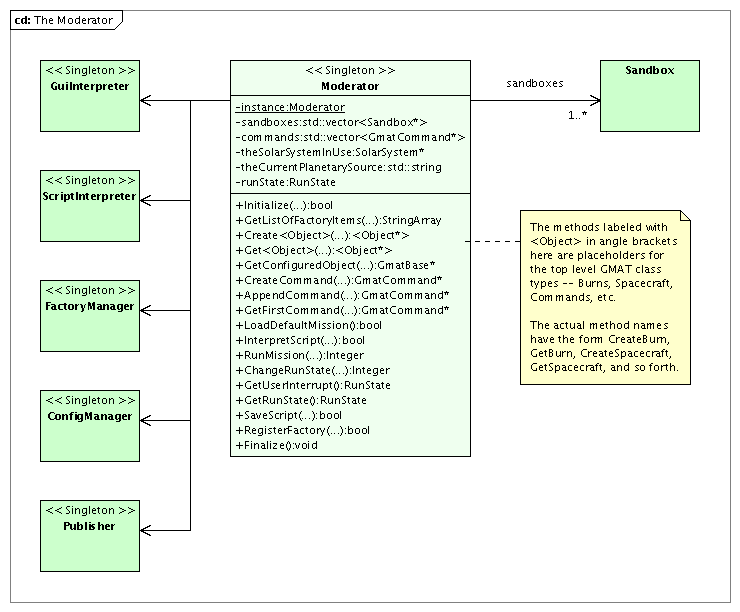
\includegraphics[370,306]{Images/TheModerator.png}
\caption{The Moderator in its Environment}
\label{figure:ModeratorClassDiagram}
\end{center}
\end{figure}

\subsection{Class Details}

The following paragraphs describe the internal data members used by
the Moderator and a brief discussion of how the methods shown in the figure are used to accomplish
its tasks.  Full details of the Moderator and its members can be found in the Doxygen
documentation, generated by running Doxygen\cite{doxygen} on GMAT's source code.

\subsubsection{Class Attributes}

There are several key data members that the Moderator uses to perform its assigned tasks.  These
members are

\begin{itemize}
\item \textbf{Moderator *instance}:  The \texttt{instance} pointer in the Moderator is the
singleton instance used throughout GMAT.
\item \textbf{std::vector<Sandbox*> sandboxes}:  GMAT's Sandbox class is used to run missions
simulating spacecraft in orbit.  The Sandbox instances are the only key players in the engine which
do not exist as singletons.  Instead, the Sandbox instances are managed by the Moderator using the
\texttt{sandboxes} vector.
\item \textbf{std::vector<GmatCommand*> commands}:  GMAT maintains a 1:1 mapping between the
Sandbox instances and the Mission Control Sequences assigned to each Sandbox.  The Moderator uses
its \texttt{commands} vector to manage the first node of the command sequence linked list for
the Mission Control Sequence of each Sandbox.
\item \textbf{SolarSystem* theSolarSystemInUse}:  GMAT's Solar System model (see
Chapter~\ref{chapter:SolarSystem}) is an aggregated object configured to include all of the bodies,
special points, and other environmental elements necessary for precision spacecraft modeling.  The
Moderator manages the Solar System used in the Sandboxes, and stores the current Solar System in
the \texttt{theSolarSystemInUse} data member.
\item \textbf{std::string theCurrentPlanetarySource}:  This string identifies the source of the
planetary ephemerides used in GMAT's environmental model.
\item \textbf{RunState runState}:  The Moderator keeps track of the current state of the Sandbox
instances in order to facilitate communications about that status between the interpreters and user
interfaces, the Publisher, and the Sandbox instances\footnote{The current implementation uses a
single runState data member.  This data structure will change to a vector when the multiple
Sandbox features of GMAT are enabled.}. The \texttt{runState} member tracks this information for the
Moderator.
\end{itemize}

Each of these class attributes plays a role in the seven tasks managed by the Moderator.
Figure~\ref{figure:ModeratorClassDiagram} also shows several methods used for these tasks.  These
methods and their roles in the Moderator's tasks are described next.

\subsubsection{Initialization and Finalization Methods}

The Moderator is responsible for starting the internal components of GMAT's engine, and for
ensuring that those components exit gracefully when GMAT is closed.  The start up process is
described in some detail in section~\ref{section:GMATStartup}.  Initialization and finalization are
performed through the following two methods:

\begin{itemize}
\item \textbf{bool Initialize(bool isFromGui = false)}:  The \texttt{Initialize} method creates the
core engine components, parses the start up file and sets up the external file pointers for
references contained in that file, and populates the Factory manager with the default factories.
This method should be called before performing any other interactions with the GMAT engine.  The
input parameter, \texttt{isFromGui}, is used to determine if the default mission should be
constructed during initialization.
\item \textbf{void Finalize()}:  The \texttt{Finalize} method is called as GMAT shuts down.  This
method frees memory that was allocated for use by the Moderator, and closes any open files managed
in the Moderator.
\end{itemize}

\subsubsection{Creation and Configuration Methods}

The creation process, described in Section~\ref{section:ObjectCreation} for configured objects and
in Section~\ref{section:CommandCreation} for commands, allocates objects and stores them in GMAT's
configuration database or the Mission Control Sequence, respectively.  These objects can then be
accessed by GMAT so that their attributes can be set as needed for the simulation, and, for the
objects in the configuration database, so that they can be copied into a Sandbox prior to a mission
run. The Moderator acts as the intermediary for the creation and object access processes, using
methods tailored to these actions.

The full set of creation and access methods are best viewed in the Doxygen files.  The following
method descriptions are representative of the full set found there.  The methods listed here use
the Burn classes to illustrate the objects that can be created in GMAT; other types of objects are
created and configured using similar methods.

\begin{itemize}
\item \textbf{StringArray GetListOfFactoryItems(Gmat::ObjectType type)}:  This method returns a
list of all of the creatable types of objects of a given supertype, described by the \texttt{type}
parameter.  For example, if the \texttt{type} parameter is set to the \texttt{BURN} type, the
returned string array contains the entries ``ImpulsiveBurn'' and ``FiniteBurn''.
\item \textbf{Burn* CreateBurn(const std::string \&type, const std::string \&name)}:  Creates a
Burn object of the specified subtype, with the specified name.  The Moderator contains creation
methods for all of GMAT's core types. These methods are all similar in form to the method shown
here; they specify the subtype and name of the requested object, and then return a pointer to the
object if it was created successfully.
\item \textbf{Burn* GetBurn(const std::string \&name)}:  Retrieves the Burn object with the
specified name.  Similar methods exist for all of GMAT's core types.
\item \textbf{GmatBase* GetConfiguredObject(const std::string \&name)}:  Returns a base class
pointer to the configured object of the specified name.
\item \textbf{GmatCommand* CreateCommand(const std::string \&type, const std::string \&name, bool
\&retFlag)}:  Creates a Mission Control Sequence command of the specified type.
\item \textbf{GmatCommand* AppendCommand(const std::string \&type, const std::string \&name, bool
\&retFlag, Integer sandboxNum = 1)}:  Creates a Mission Control Sequence command of the specified
type, and passes it into the Mission Control Sequence associated with the specified Sandbox.
\item \textbf{GmatCommand* GetFirstCommand(Integer sandboxNum = 1)}:  Retrieves the first command
in the Mission Control Sequence associated with the specified Sandbox.  Since the Mission Control
Sequence is a linked list, this method can be used to retrieve the entire Mission Control Sequence.
\end{itemize}

\subsubsection{Reading or Saving a Mission}

The processes followed when loading a mission into GMAT and when saving a mission from GMAT are
managed by the Script Interpreter.

The read process is implemented as a sequence of object creations and configurations in the
Script Interpreter.  The Moderator passes requests for these processes to the Interpreter through
several different methods, including these:

\begin{itemize}
\item \textbf{bool LoadDefaultMission()}:  Clears the current configuration and Mission Control
Sequence from memory, and then creates and configures the default GMAT mission.
\item \textbf{bool InterpretScript(const std::string \&filename, bool readBack = false, const
std::string \&newPath = "")}:  Creates and configures all of the objects in a script file.
\end{itemize}

Each object defining a mission in GMAT includes the ability to serialize itself so that is can be
passed to an external process or written to a file.  The Moderator passes requests for this
serialization to the Script Interpreter for processing.  A representative example of the Moderator
methods used for this process is the \texttt{SaveScript} method:

\begin{itemize}
\item \textbf{bool SaveScript(const std::string \&filename, Gmat::WriteMode mode =
Gmat::SCRIPTING)}:  Builds scripts from the configured objects and commands, and write them to a
file named by the \texttt{filename} parameter.  The writeMode parameter is used to determine the
style of the serialization; it can be set to either the default \texttt{SCRIPTING} style or to a
style, \texttt{MATLAB\_STRUCT}, compatible with MATLAB.
\end{itemize}

\noindent Details of the actual processes followed when reading or writing a script can be found in
Chapter~\ref{chapter:ScriptRW}.

\subsubsection{Methods Used to Run a Mission}

The process followed when GMAT runs a mission is described in
Section~\ref{section:SandboxMCSExecution}.  The process is relatively straightforward: the
configured objects and Mission Control Sequence are loaded into the Sandbox instance, initialized
to establish the connections between those objects, and then run in the Sandbox, as described in
Section~\ref{section:SandboxMCSExecution} and in Chapter~\ref{chapter:Sandbox}.  The Moderator
supports these tasks through the following methods and through similar methods that can be examined
in the Doxygen output.

\begin{itemize}
\item \textbf{Integer RunMission(Integer sandboxNum = 1)}:  Loads objects into the specified
Sandbox, initializes it, and starts the mission run in the Sandbox.
\item \textbf{Integer ChangeRunState(const std::string \&state, Integer sandboxNum = 1)}: 
Method used by the interpreters to update the run state information in the Moderator, so that the
Sandbox can later check the Moderator's run state.
\item \textbf{RunState GetUserInterrupt()}:  Method called to determine if the user has requested a
change in the run state.  This method queries the interpreter for state changes before returning
the run state, so that the interpreter code has an opportunity to update the state based on user
actions.
\item \textbf{RunState GetRunState()}:  Returns the current run state of the Sandbox.
\end{itemize}

The Moderator keeps track of the state of execution in the Sandbox instance so that it can respond
to messages from the interpreters that affect the system, like user commands to pause or terminate
the run.  The discussion in Section~\ref{section:SandboxMCSExecution} presented the program flow
exercised during a mission run.  During the loop through the Mission Control Sequence shown in
Figure~\ref{figure:RunningBasicScript}, the Sandbox polls the Moderator for the execution state.
This polling checks the Moderator's state variable and responds accordingly, as discussed in
Chapter~\ref{chapter:Sandbox}.

\begin{figure}[htb]
\begin{center}
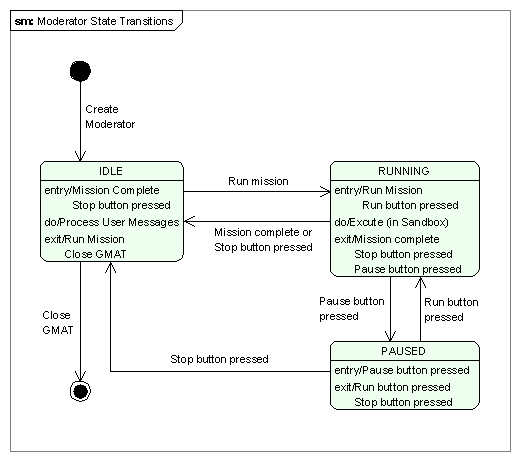
\includegraphics[260,231]{Images/ModeratorStateTransitions.png}
\caption{State Transitions in the Moderator}
\label{figure:ModeratorStateTransitions}
\end{center}
\end{figure}

\subparagraph{\label{section:ModeratorStates}\textit{State Transitions in the Moderator}}

The Moderator tracks the current state of the system using a parameter named runState, which is set
to a value in the RunState enumeration (see Table~\ref{table:RunStateEnum}) defined in the Gmat
namespace.  The engine states tracked in the Moderator are the IDLE, RUNNING, and PAUSED states.

Figure ~\ref{figure:ModeratorStateTransitions} shows the run state transitions tracked by the
Moderator.  The Moderator is created with the run state set to the IDLE state.  Most of the time,
the Moderator remains in the IDLE state, processing messages from users and managing the internal
components of the GMAT engine\footnote{Many of the activities performed by the Moderator in the IDLE
state are described in Chapter~\ref{chapter:TopLevel}.  Additional Moderator interactions with the
other engine components are described in the appropriate sections of this document.}.

When a user executes a Mission Control Sequence, the Moderator transitions to the RUNNING state.  In
this state, the Moderator performs very limited processing while the control of the system is
managed by the sandbox that is running the mission.  The sandbox polls the Moderator for user
activity at convenient points during the mission run.  This polling allows the Moderator to respond
to user actions that either terminate the mission early or pause the mission.

If the user presses the pause button on the GUI, the Moderator transitions into the PAUSED state
when the sandbox polls for state status.  This activity stops the mission run, but maintains data so
that the run can be resumed from the point of the stop.  The user tells the Moderator to resume the
run by pressing the run button on the GUI.  When the Moderator receives the run message, it
transitions back into the RUNNING state and tells the sandbox to resume the run.

The user can terminate a run early by pressing the stop button on the GUI during a run.  This action
always causes the Moderator to transition from its current state - either RUNNING or PAUSED -- into
the IDLE state.

\subsubsection{Support for Extending GMAT}

GMAT employs a design pattern that allows the objects and commands used in simulations to be
treated generically in the engine code.  The system can be extended by creating a class or
collection of classes, derived from one of GMAT's base classes, for each new feature that is added
to the system, and then creating a Factory class that constructs instances of these new classes. 
This Factory is registered with GMAT's Factory Manager through the following call in the Moderator: 

\begin{itemize}
\item \textbf{bool RegisterFactory(Factory* newFactory)}:  Adds a Factory to the object creation
subsystem managed by the Factory Manager.
\end{itemize}

\noindent  Further details of the Factory subsystem can be found in
Chapter~\ref{chapter:FactoryManager}.

\section{Usage and Modification}

The Moderator runs in the background for most of GMAT's programmatic tasks.  You'll need to
interact with it directly if you are working with the Factory Manager, Configuration Manager, or
Sandbox code, or if you are adding a new interface to GMAT that requires a new Interpreter.  Most
programmatic tasks are not that extensive, and can be performed without changing the Moderator.

If you are adding a new user class to GMAT, you'll need to register the factory that creates
instances of that class.  These extensions are made through a call to the Moderator's
\texttt{RegisterFactory} method, as described in Chapter~\ref{chapter:ExtendingGMAT}.  In addition,
if the new class is not derived from a base class matching the set of Create and Get functions in
the Moderator, you may need to add these methods to the Moderator code\footnote{The GMAT
development team has this item noted as an issue that needs to be resolved.}.

By design, the Moderator was written to support operations in GMAT's engine as it stands without
the need for further extension.  If you find a case that seems to need new functionality in the
Moderator, please start a discussion regarding the change on GMAT's message forums at
SourceForge\footnote{http://sourceforge.net/projects/gmat}.
